% \documentclass[aspectratio=169, 11pt]{beamer}
\documentclass[aspectratio=169, 11pt, handout]{beamer}
 
% ── Theme ──
\usetheme{Madrid}
\usecolortheme{default}
\setbeamertemplate{navigation symbols}{}
\setbeamertemplate{footline}{%
  \leavevmode\hbox{%
    \begin{beamercolorbox}[wd=.333333\paperwidth,ht=2.5ex,dp=1ex,center]{author in head/foot}%
      \usebeamerfont{author in head/foot}\insertshortauthor
    \end{beamercolorbox}%
    \begin{beamercolorbox}[wd=.333333\paperwidth,ht=2.5ex,dp=1ex,center]{title in head/foot}%
      \usebeamerfont{title in head/foot}\insertshorttitle
    \end{beamercolorbox}%
    \begin{beamercolorbox}[wd=.333333\paperwidth,ht=2.5ex,dp=1ex,right]{date in head/foot}%
      \usebeamerfont{date in head/foot}\insertframenumber{} / \inserttotalframenumber\hspace*{2ex}
    \end{beamercolorbox}}}
 
% ── Packages ──
\usepackage{amsmath,amssymb}
\usepackage{booktabs}
\usepackage{xcolor}
\usepackage{colortbl}
\usepackage{tikz}
\usetikzlibrary{arrows.meta, positioning, calc}
 
% ── Colors ──
\definecolor{sbgreen}{HTML}{00704A}  % Starbucks green
\definecolor{warnred}{HTML}{CC0000}
\definecolor{noteblue}{HTML}{2060A0}
 
% ── Commands ──
\newcommand{\E}{\mathbb{E}}
\newcommand{\Var}{\mathrm{Var}}
\newcommand{\SE}{\mathrm{SE}}
\newcommand{\Prob}{\mathrm{Pr}}
\newcommand{\indep}{\perp\!\!\!\perp}

% ── Title ──
\title[Lecture 1]{Lecture 1: The Counterfactual Framework}
\subtitle{Applied ML for Business Part II}
\author{Zhikun Lu}
\date{\today}

\begin{document}

% ====================================================================
\begin{frame}
\titlepage
\end{frame}

% ====================================================================
\begin{frame}{Module 3 Roadmap}

\begin{center}
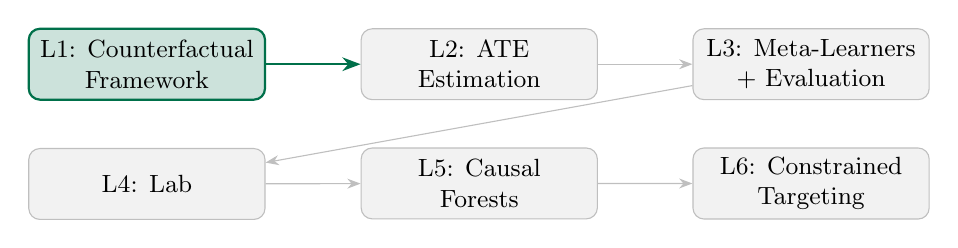
\begin{tikzpicture}[
    node distance=0.6cm and 1.2cm,
    box/.style={draw, rounded corners, minimum width=3cm, minimum height=0.9cm, font=\small, align=center},
    active/.style={box, fill=sbgreen!20, draw=sbgreen, thick},
    inactive/.style={box, fill=gray!10, draw=gray!50}
]
\node[active] (L1) {L1: Counterfactual\\Framework};
\node[inactive, right=of L1] (L2) {L2: ATE\\Estimation};
\node[inactive, right=of L2] (L3) {L3: Meta-Learners\\+ Evaluation};
\node[inactive, below=of L1] (L4) {L4: Lab};
\node[inactive, below=of L2] (L5) {L5: Causal\\Forests};
\node[inactive, below=of L3] (L6) {L6: Constrained\\Targeting};

\draw[-{Stealth}, thick, sbgreen] (L1) -- (L2);
\draw[-{Stealth}, gray!50] (L2) -- (L3);
\draw[-{Stealth}, gray!50] (L3) -- (L4);
\draw[-{Stealth}, gray!50] (L4) -- (L5);
\draw[-{Stealth}, gray!50] (L5) -- (L6);
\end{tikzpicture}
\end{center}
\end{frame}

% ====================================================================
\begin{frame}{Today's Plan}

\begin{enumerate}
    \item The Starbucks coupon problem (recap + new material)
    \item Potential outcomes and the four customer types
    \item Why naive comparisons fail: confounding
    \item The solution: randomization
    \item Hypothesis testing: is the difference real?
    \item When randomization is impossible
\end{enumerate}

\bigskip
\textbf{Reading:} Chapters 1--2 of the textbook.
\end{frame}

% ====================================================================
\section{The Starbucks Problem}
% ====================================================================

\begin{frame}{The Setup}

\textbf{Starbucks} has 10,000 customers in its loyalty database.

\bigskip

The marketing team wants to send a coupon (\textyen 10 off next purchase).

\bigskip

\textbf{The question:} Which customers should receive the coupon?

\bigskip

\begin{itemize}
    \item Each coupon costs \textyen 10 if redeemed
    \item Each purchase generates \textyen 30 margin (20 if a coupon redeemed)
    \item Sending to everyone: profitable only if the coupon \emph{causes} enough extra purchases
\end{itemize}
\end{frame}

% ====================================================================
\begin{frame}{The Prediction Approach (and Why It Fails)}

\textbf{Natural idea:} Build a model to predict who will buy, then send coupons to high-probability customers.

\bigskip
\pause

\textbf{Problem:} The model predicts $\Prob(\text{purchase} \mid X)$, not the \emph{causal effect} of the coupon.

\bigskip

\begin{center}
\begin{tabular}{lcc}
\toprule
\textbf{Customer} & \textbf{P(buy)} & \textbf{Effect of coupon} \\
\midrule
Daily regular & 0.95 & $\approx 0$ (buys anyway) \\
Lapsed customer & 0.05 & could be large \\
\bottomrule
\end{tabular}
\end{center}

\bigskip

Prediction targets the \emph{wrong column}. We need the \emph{missing column}: the causal effect.
\end{frame}

% ====================================================================
\begin{frame}{The Four Types of Customers}

For each customer, imagine \textbf{two worlds}: one with coupon, one without.

\bigskip

\begin{center}
\begin{tabular}{l|c|c|}
\multicolumn{1}{c}{} & \multicolumn{1}{c}{\textbf{Doesn't buy with coupon}} & \multicolumn{1}{c}{\textbf{Buys with coupon}} \\
\cline{2-3}
\textbf{Doesn't buy without} & \cellcolor{gray!15} Lost Cause & \cellcolor{green!15} \textbf{Persuadable} \\
& ITE $= 0$ & ITE $= +1$ \\
\cline{2-3}
\textbf{Buys without} & \cellcolor{red!15} Do-Not-Disturb & \cellcolor{blue!10} Sure Thing \\
& ITE $= -1$ & ITE $= 0$ \\
\cline{2-3}
\end{tabular}
\end{center}

\bigskip
\pause

\begin{itemize}
    \item \textbf{Persuadable:} coupon \emph{causes} purchase $\longrightarrow$ profit!
    \item \textbf{Sure Thing:} buys anyway $\longrightarrow$ coupon is wasted money
    \item \textbf{Lost Cause:} doesn't buy regardless $\longrightarrow$ coupon is wasted
    \item \textbf{Do-Not-Disturb:} coupon \emph{hurts} $\longrightarrow$ avoid!
\end{itemize}
\end{frame}

% ====================================================================
\begin{frame}{The Fundamental Problem}

\begin{alertblock}{Key Insight}
For each customer, we observe \textbf{only one} of the two worlds.
\end{alertblock}

\bigskip

\begin{itemize}
    \item If customer $i$ gets the coupon, we see whether they buy \emph{with} the coupon
    \item We \textbf{never} see what they would have done \emph{without} it
    \item The other outcome is the \textbf{counterfactual}
\end{itemize}

\bigskip
\pause

This means:
\begin{itemize}
    \item We cannot classify any individual into one of the four types
    \item We need a strategy that works at the \emph{population} level
\end{itemize}
\end{frame}

% ====================================================================
\section{Potential Outcomes}
% ====================================================================

\begin{frame}{Formalizing Counterfactuals}

\textbf{Notation.} For each individual $i$:

\bigskip

\begin{tabular}{ll}
$D_i \in \{0, 1\}$ & treatment assignment (1 = coupon, 0 = no coupon) \\[0.3em]
$Y_i(1)$ & \textbf{potential outcome} if treated \\[0.3em]
$Y_i(0)$ & \textbf{potential outcome} if not treated \\[0.3em]
$\tau_i = Y_i(1) - Y_i(0)$ & \textbf{individual treatment effect} (ITE)
\end{tabular}

\bigskip
\pause

\textbf{Observed outcome:}
\[
Y_i = D_i \cdot Y_i(1) + (1 - D_i) \cdot Y_i(0)
\]

We see $Y_i(1)$ if treated, $Y_i(0)$ if not. Never both.

\bigskip

\textbf{Average treatment effect (ATE):}
\[
\tau = \E[Y(1) - Y(0)] = \Prob(\text{Persuadable}) - \Prob(\text{Do-Not-Disturb})
\]
\end{frame}

% ====================================================================
\begin{frame}{A Harder Example: The George Floyd Case}

\begin{quote}
Would the outcome have been different if George Floyd had been perceived as white?
\end{quote}

\pause
\medskip

The same framework applies:
\begin{itemize}
    \item $D = 1$: perceived as Black; $D = 0$: perceived as White
    \item $Y(1)$: outcome under Black perception; $Y(0)$: outcome under White perception
    \item ITE: $Y(1) - Y(0)$
\end{itemize}

\medskip
\pause

Same four types:
\begin{center}
\small
\begin{tabular}{ll}
\textbf{Type 1:} & Survives regardless (ITE $= 0$) \\
\textbf{Type 2:} & Dies regardless (ITE $= 0$) \\
\textbf{Type 3:} & Dies because of race (ITE $= +1$) \\
\textbf{Type 4:} & Survives because of race (ITE $= -1$) \\
\end{tabular}
\end{center}

\medskip

Floyd: observed $D = 1$, $Y = 1$. He is Type 2 or Type 3. \textbf{We cannot tell which.}
\end{frame}

% ====================================================================
\section{Confounding}
% ====================================================================

\begin{frame}{The Naive Comparison and Why It Fails}

\textbf{Natural idea:} Compare outcomes between treated and untreated groups.

\bigskip

\[
\text{``Effect''} = \E[Y \mid D = 1] - \E[Y \mid D = 0]
\]

\bigskip
\pause

\textbf{Problem:} This equals the ATE \emph{only if} the groups are comparable.

\bigskip

If the marketing team targets coupons at loyal customers:
\begin{itemize}
    \item Coupon group: packed with \textbf{Sure Things} (buy anyway)
    \item No-coupon group: more \textbf{Lost Causes} (don't buy anyway)
    \item The coupon \emph{looks} effective, but the groups were different to begin with
\end{itemize}

\bigskip

This is \textbf{confounding}: a variable (loyalty) affects both treatment and outcome.
\end{frame}

% ====================================================================
\begin{frame}{Confounding: A Numerical Example}

True type distribution: 1,000 customers.

\begin{center}
\small
\begin{tabular}{lrc}
\toprule
\textbf{Type} & \textbf{Count} & \textbf{Share} \\
\midrule
Lost Cause (0,0) & 400 & 40\% \\
Sure Thing (1,1) & 300 & 30\% \\
Persuadable (0,1) & 200 & 20\% \\
Do-Not-Disturb (1,0) & 100 & 10\% \\
\bottomrule
\end{tabular}
\end{center}

True ATE $= 0.50 - 0.40 = \mathbf{0.10}$ (10 pp).
\end{frame}

% ====================================================================
\begin{frame}{Confounded Assignment}

Marketing targets 500 loyal customers $\Rightarrow$ Sure Things overrepresented in coupon group:

\begin{center}
\small
\begin{tabular}{lccr}
\toprule
\textbf{Type} & \textbf{Coupon (500)} & \textbf{No-coupon (500)} & \textbf{Total} \\
\midrule
Lost Cause (0,0) & 100 & 300 & 400 \\
Sure Thing (1,1) & \textcolor{warnred}{220} & 80 & 300 \\
Persuadable (0,1) & 120 & 80 & 200 \\
Do-Not-Disturb (1,0) & 60 & 40 & 100 \\
\bottomrule
\end{tabular}
\end{center}

\pause

\begin{align*}
\text{Purchase rate (coupon)} &= (220 + 120)/500 = 0.68 \\
\text{Purchase rate (no-coupon)} &= (80 + 40)/500 = 0.24 \\
\text{Naive difference} &= 0.68 - 0.24 = \textcolor{warnred}{0.44}
\end{align*}

\textbf{4.4$\times$ the true effect!} Sure Things inflate the coupon group's success rate.
\end{frame}

% ====================================================================
\section{Randomization}
% ====================================================================

\begin{frame}{The Solution: Randomization}

Randomly assign 500 customers to coupon, 500 to control.

\begin{center}
\small
\begin{tabular}{lccr}
\toprule
\textbf{Type} & \textbf{Coupon (500)} & \textbf{No-coupon (500)} & \textbf{Total} \\
\midrule
Lost Cause (0,0) & 200 & 200 & 400 \\
Sure Thing (1,1) & \textcolor{sbgreen}{150} & \textcolor{sbgreen}{150} & 300 \\
Persuadable (0,1) & 100 & 100 & 200 \\
Do-Not-Disturb (1,0) & 50 & 50 & 100 \\
\bottomrule
\end{tabular}
\end{center}

\pause

\begin{align*}
\text{Purchase rate (coupon)} &= (150 + 100)/500 = 0.50 \\
\text{Purchase rate (no-coupon)} &= (150 + 50)/500 = 0.40 \\
\text{Difference} &= 0.50 - 0.40 = \textcolor{sbgreen}{\mathbf{0.10}} = \text{true ATE} \; \checkmark
\end{align*}
\end{frame}

% ====================================================================
\begin{frame}{Why Randomization Works}

Three properties:

\bigskip

\begin{enumerate}
    \item Balances \textbf{observable} confounders (loyalty tier, purchase history, \ldots)
    
    \bigskip
    
    \item Balances \textbf{unobservable} confounders (just got a raise, competitor opened nearby, \ldots)
    
    \bigskip
    
    \item Makes $\bar{Y}_{\text{coupon}} - \bar{Y}_{\text{no-coupon}}$ an \textbf{unbiased estimator} of the ATE:
    \[
    \E\!\left[\bar{Y}_1 - \bar{Y}_0\right] = \tau
    \]
\end{enumerate}

\bigskip

This is a \textbf{randomized controlled trial} (RCT), or in business: an \textbf{A/B test}.
\end{frame}

% ====================================================================
\section{Hypothesis Testing}
% ====================================================================

\begin{frame}{Is the Difference Real or Just Noise?}

Even under the null (coupon has \emph{no} effect), random assignment will produce \emph{some} difference.

\medskip

\textbf{Question:} How unlikely is a difference of 0.10 if the truth is 0?

\medskip
\pause

\textbf{Fisher's Lady Tasting Tea (1935):}
\begin{itemize}
    \item Colleague Muriel Bristol claimed she could tell whether tea or milk was poured first
    \item Fisher prepared 8 cups (4 each), random order
    \item Bristol got all 8 correct
    \item Under null (guessing): $\binom{8}{4} = 70$ possible assignments, only 1 all-correct
    \item P-value $= 1/70 \approx 0.014$
\end{itemize}

\medskip

\begin{block}{P-value}
The probability of a result at least as extreme as what we observed, \textbf{assuming the null is true}.
\end{block}
\end{frame}

% ====================================================================
\begin{frame}{Mapping Tea onto Starbucks}

\begin{center}
\begin{tabular}{ll}
\toprule
\textbf{Lady Tasting Tea} & \textbf{Starbucks A/B Test} \\
\midrule
8 cups & 1,000 customers \\
4 milk-first, 4 tea-first (fixed) & 450 purchasers, 550 non-purchasers (fixed under null) \\
Bristol labels 4 cups ``milk-first'' & Randomization assigns 500 to coupon group \\
Labels are random (under null) & Treatment assignment is random (by design) \\
\bottomrule
\end{tabular}
\end{center}

\bigskip
\pause

Under the null: outcomes are \textbf{fixed}, labels are the \textbf{only random element}.

\bigskip

Any observed difference is just the luck of the draw.
\end{frame}

% ====================================================================
\begin{frame}{The Urn Model}

Think of the data as an \textbf{urn}: 450 balls labeled ``1'' and 550 labeled ``0.''

\bigskip

Under the null, these labels are \textbf{fixed}. Random assignment draws 500 into treatment.

\bigskip

Expected 1's in each group: $500 \times 450/1000 = 225$. So $\E[\bar{Y}_1 - \bar{Y}_0] = 0$.

\bigskip
\pause

By the CLT, $\bar{Y}_1 - \bar{Y}_0$ is approximately normal. Using the \textbf{pooled proportion} $\hat{p} = 0.45$:

\[
\SE_0 = \sqrt{\frac{2\hat{p}(1-\hat{p})}{500}} \approx 0.0315, \qquad z = \frac{0.10}{0.0315} \approx 3.17, \qquad \text{p-value} \approx 0.0015
\]

\bigskip

Reject $H_0$. But this formula \textbf{assumes the null is true} (pooled $\hat{p}$). In practice, we want an approach that works without assuming the null and generalizes to continuous outcomes.
\end{frame}

% ====================================================================
\begin{frame}{The Modern Approach: Three Facts}

We observed $\hat{\tau} = \bar{Y}_1 - \bar{Y}_0 = 0.10$. How precise is this estimate?

\bigskip

\textbf{Fact 1:} Variance of a sample mean is $\sigma^2 / n$.
\[
\Var(\bar{Y}_1) = \frac{0.50 \times 0.50}{500} = 0.0005, \qquad \Var(\bar{Y}_0) = \frac{0.40 \times 0.60}{500} = 0.00048
\]

\pause

\textbf{Fact 2:} Independent variances add. (Random assignment ensures $\bar{Y}_1 \indep \bar{Y}_0$.)
\[
\Var(\hat{\tau}) = 0.0005 + 0.00048 = 0.00098, \qquad \widehat{\SE} = \sqrt{0.00098} \approx 0.0313
\]

\pause

\textbf{Fact 3:} CLT $\Rightarrow$ $\hat{\tau}$ is approximately normal.

\bigskip

No null hypothesis was invoked. We simply asked: \textbf{how much would $\hat{\tau}$ fluctuate} if we reran the experiment?
\end{frame}

% ====================================================================
\begin{frame}{Testing and Confidence Interval}

\begin{block}{Hypotheses}
$H_0$: $\tau = 0$ (coupon has no average effect) \qquad $H_1$: $\tau \neq 0$
\end{block}

\medskip

The $z$-statistic: how many standard errors is our estimate from zero?
\[
z = \frac{\hat{\tau}}{\widehat{\SE}} = \frac{0.10}{0.0313} \approx 3.19 \qquad \text{p-value} \approx 0.0014
\]

\pause

\textbf{Reject} $H_0$ at 5\% level. The coupon has a real effect.

\medskip

95\% confidence interval:
\[
\hat{\tau} \pm 1.96 \times \widehat{\SE} = 0.10 \pm 0.061 = [0.039, \; 0.161]
\]

\begin{itemize}
    \item The true effect is between about 4 and 16 percentage points
    \item If we reran this experiment many times, $\sim$95\% of the CIs would contain $\tau$
\end{itemize}
\end{frame}

% ====================================================================
\begin{frame}{Two Approaches, Same Conclusion}

\begin{center}
\small
\begin{tabular}{lcc}
\toprule
& \textbf{Urn / Fisher} & \textbf{Modern (two-sample)} \\
\midrule
SE computation & Pooled $\hat{p}$ under null & Each group's own $\hat{p}$ \\
$z$-statistic & 3.17 & 3.19 \\
p-value & 0.0015 & 0.0014 \\
Assumes null? & Yes (for SE) & No \\
Gives CI? & Not directly & Yes \\
Continuous outcomes? & Needs modification & Works as-is \\
\bottomrule
\end{tabular}
\end{center}

\medskip

Results are nearly identical here. The modern approach is what A/B test platforms (Netflix, Uber, Alibaba) use in practice.

\medskip

\begin{block}{Takeaway}
The p-value tells you whether the difference is \textbf{distinguishable from noise}. The confidence interval tells you \textbf{how big} the effect plausibly is. Always report both.
\end{block}
\end{frame}

% ====================================================================
\section{When Randomization Fails}
% ====================================================================

\begin{frame}{Back to Floyd: The Manipulability Problem}

We cannot randomly assign perceived race.

\bigskip

The obstacle is \textbf{conceptual}, not just practical:
\begin{itemize}
    \item ``Change Floyd's race but hold everything else fixed''
    \item What does it mean for Floyd to be perceived as White?
    \item Same neighborhood? Same life experiences?
    \item The counterfactual may not be \textbf{well-defined}
\end{itemize}

\bigskip
\pause

\begin{block}{Holland's Dictum}
``No causation without manipulation.'' Causal effects are well-defined only when the treatment could, in principle, be experimentally varied.
\end{block}
\end{frame}

% ====================================================================
\begin{frame}{The Solution: Randomize a Signal}

We cannot assign race. We \emph{can} assign a \textbf{signal} of race.

\bigskip

\textbf{Bertrand \& Mullainathan (2004, American Economic Review):}
\begin{itemize}
    \item Sent identical resumes to job ads in Boston and Chicago
    \item Only difference: name (``Emily Walsh'' vs.\ ``Lakisha Washington'')
    \item Name was \textbf{randomly assigned}
    \item Result: White-sounding names got \textbf{50\% more callbacks}
\end{itemize}

\bigskip
\pause

\textbf{Cui, Li, \& Zhang (2019, \emph{Management Science}):}
\begin{itemize}
    \item Confirmed racial discrimination on Airbnb (audit study)
    \item Then tested an intervention: positive reviews from prior hosts
    \item Result: gap \textbf{disappeared} when credible quality signal was present
\end{itemize}
\end{frame}

% ====================================================================
\begin{frame}{A Taxonomy of Causal Questions}

\begin{center}
\small
\begin{tabular}{p{2.5cm}p{3cm}p{4.5cm}p{2cm}}
\toprule
\textbf{Type} & \textbf{Example} & \textbf{What makes it hard} & \textbf{Our focus} \\
\midrule
Manipulable treatment & Coupon, price, drug & Execution: sample size, compliance & \textcolor{sbgreen}{\textbf{Core}} \\[0.5em]
Policy variable & Education, tax rate & Bundling: changes many things & Partial \\[0.5em]
Attribute variable & Race, gender & Conceptual: counterfactual unclear & Discussed \\[0.5em]
System-level & ``What if Uber never existed?'' & Undefined treatment & Out of scope \\
\bottomrule
\end{tabular}
\end{center}

\bigskip

\textbf{This course:} manipulable treatments (coupons, prices) where A/B testing is feasible.
\end{frame}

% ====================================================================
\begin{frame}{Key Takeaways}

\begin{enumerate}
    \item \textbf{Causal inference = reconstructing missing counterfactuals.} The four types define what ``causal'' means at the individual level.
    
    \bigskip
    
    \item \textbf{Confounding distorts naive comparisons.} When treatment assignment correlates with potential outcomes, simple group comparisons are biased.
    
    \bigskip
    
    \item \textbf{Randomization is the gold standard.} It balances observed \emph{and} unobserved confounders.
    
    \bigskip
    
    \item \textbf{Not all causal questions are well-defined.} Before asking ``what is the effect of $X$?'', ask: is $X$ a manipulable intervention?
\end{enumerate}

\bigskip

\textbf{Next time:} Formalizing the ATE, selection bias decomposition, estimation, and the transition to heterogeneous effects.
\end{frame}

\end{document}